\subsection{Front-end Arkitektur}

Front-end applikationen er det man kan kalde, brugerens vindue til spillet. Det er i dette modul at brugeren vil få alt sit information
og vil få mulighed for at lave inputs til spillet. 
Front-end'en er opbygget af et hav af forskellige skærme og menuer, og for at give et overblik over disse er der lavet følgende C3 model
for Front-end'en (\autoref{fig:Arkitektur-FrontEnd-C3}), som giver en idé om hvilke skærme og menuer der kan gå til hvilke andre menuer/skærme.
Udover dette fortæller modellen også om hvordan og hvilke skærme og menuer der snakker med noget uden for Front-end'en selv, f.eks. skal der
ved Login/Register kontaktes databasen for at få verificeret logind-oplysninger, og samtidig skal der ved save og load-game hentes en liste af
gemte spil i databasen, hvorefter der skal henholdsvis skrives og hentes fra databasen alt efter om man gemmer eller henter et spil.

\begin{figure}[H]
\centering
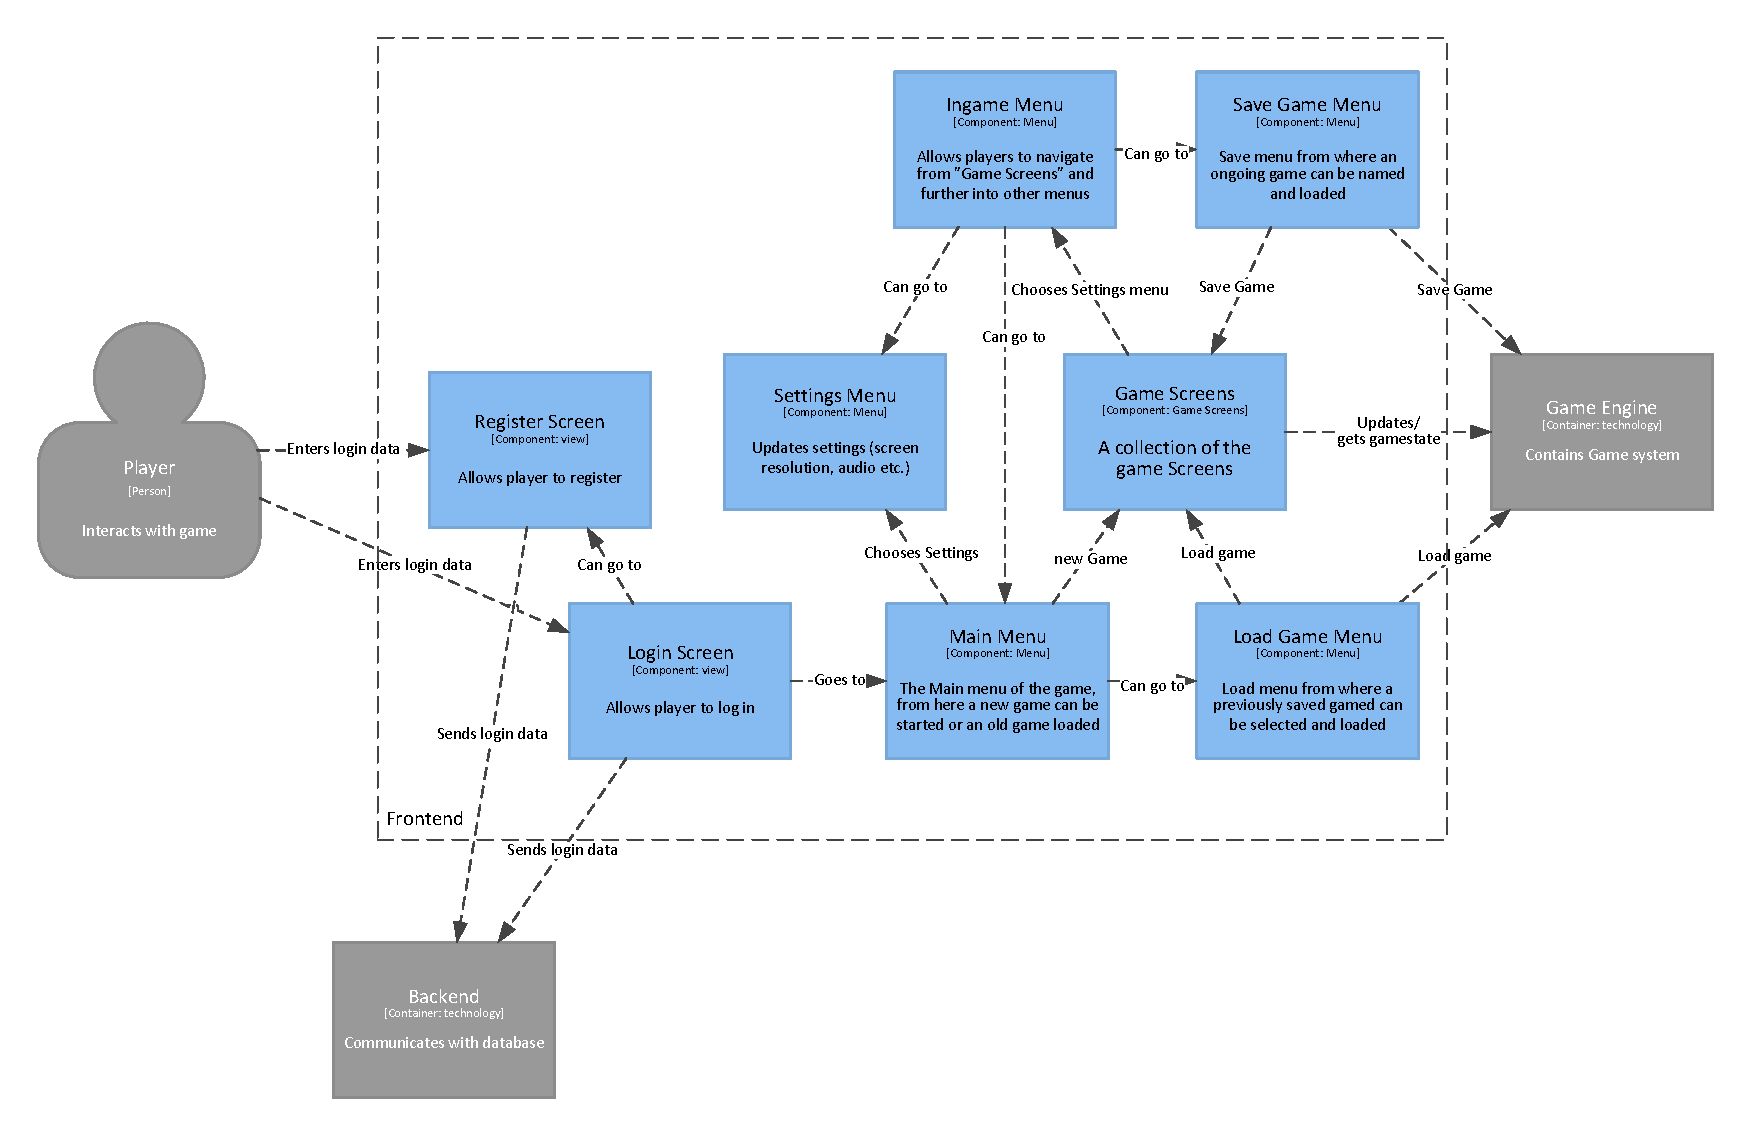
\includegraphics[width = \textwidth]{02-Body/Images/Frontend_C3.pdf}
\caption{C3-Model for Front-end. Modellen fortæller hvordan man kan navigere igennem forskellige menuer og hvilke menuer der kan føre til hvad. Derudover kan man se hvilke blokke der snakker ud af front-end'en og sammen med resten af systemet.}
\label{fig:Arkitektur-FrontEnd-C3}
\end{figure}

\subsubsection{Pseudo Front-end Arkitektur}
For at give overblik over, hvordan kommunikationen mellem frontend, backend og gamecontroller kommer til at foregå, er der lavet et pseudo sekvensdiagram for følgende UserStories:
\\
- Login\\
- Register\\
- Save Game\\
- Load Game\\

<<<<<<< HEAD
Der vil i dette afsnit kun blive vist "Save Game". "Load Game","Login" og "Register" kan findes i Teknisk Bilag \parencite[][Section 9.2.1]{TekniskBilag}.
=======
Der vil i dette afsnit kun blive vist "Save Game". "Load Game","Login" og "Register" kan findes i Tekniskbilag (sektion 7.2.1).
>>>>>>> e7730d420e4c7e2d210d5ddee06828ffbe89fe67

\noindent På \autoref{fig:Arkitektur-FrontEnd-Save} ses "Save Game", som viser forløbet når en bruger gerne vil gemme sit igangværende spil, set fra Frontends perspektiv. 
Hertil skal der nævnes at hvis brugeren er i "Combat State" er det ikke muligt at gemme spillet og knappen "Save Game" på "In Game Menu" vil ikke kunne ses eller bruges.\\

\begin{figure}[H]
\centering
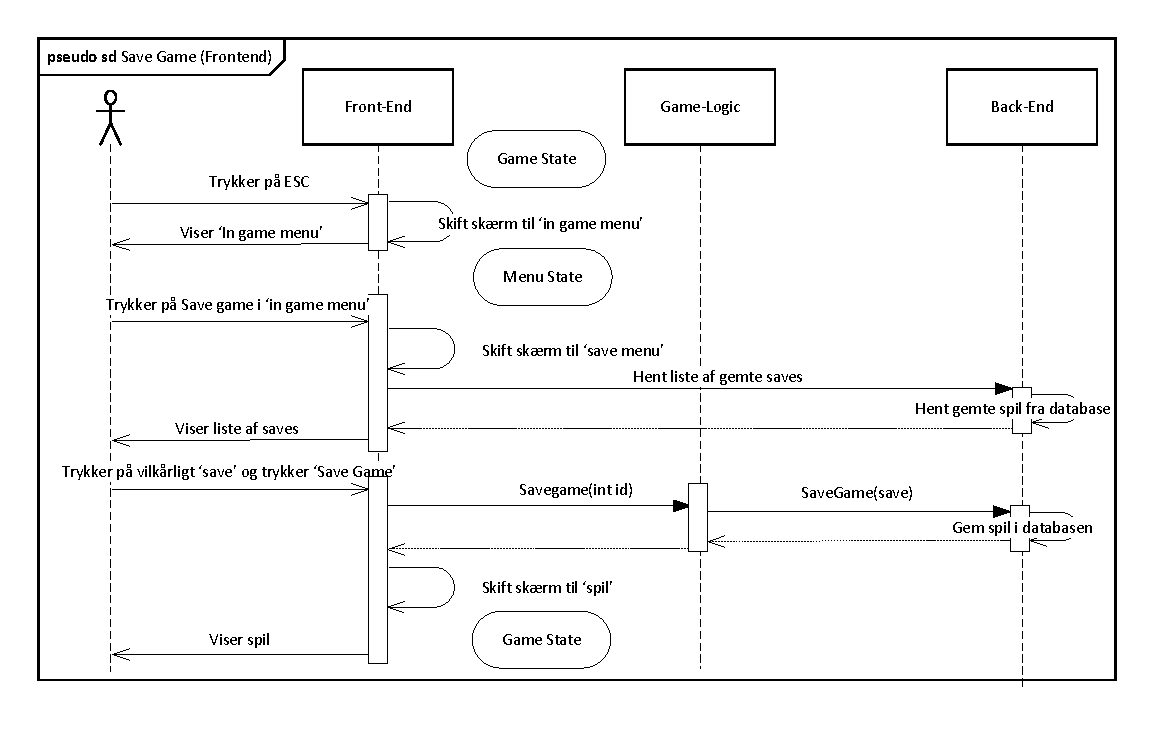
\includegraphics[width = \textwidth]{02-Body/Images/Front-End_-_Arkitektur-savegame.pdf}
\caption{Pseudo sekvensdiagram af forløbet af userstory "Save Game", set fra Frontends perspektiv. Der laves 2 kald til databasen igennem Backenden, hvori der i det første kald,  "Hent liste af gemte saves" hentes en liste af brugerens gemte spil og i andet kald gemmes brugerens nuværende spil henover det valgte spil.}
\label{fig:Arkitektur-FrontEnd-Save}
\end{figure}

\newpage
